% Figure 12 supplementary-material insert for the v2.1.0 development gate.
% The published v2.0.0 supplement and accepted source-v1 paper remain frozen.

\subsection{Fixed-time order-book shock recovery}
\label{app:fixed-time-shock-recovery}

Figure~\ref{fig:fixed-time-shock-recovery} follows one buy market order in
book 1 through the current fixed-grid operational dynamics.  Immediately
before the declared operational step, the order consumes opposing density
from the reaction boundary outwards.  If $M_{1,n_*}$ denotes the resulting
density increment, then
\begin{equation}
  \varphi^+_{1,n_*}=\varphi^-_{1,n_*}+M_{1,n_*},
  \qquad
  \Delta x\sum_i |M_{1,n_*,i}|=Q.
\end{equation}
The event is applied once and only to book 1.  The second book remains active
through the receiving-front translation-mode coupling, although its density
and the coupling contribution are not separately drawn.

For a completed operational step the stored density satisfies
\begin{equation}
  \varphi_{j,n+1}
  =H_{j,n}+\varphi^+_{j,n}+C_{j,n}+A_{j,n}+L_{j,n}+B_{j,n},
\end{equation}
where $H$ is the transport or memory contribution,
\begin{equation}
  A_{j,n}=\Delta u\,q_j,
  \qquad
  C_{j,n}=\left(e^{-\nu_j\Delta u}-1\right)\varphi^+_{j,n},
  \qquad
  L_{j,n}=\Delta u\,\ell_{j\leftarrow k},
\end{equation}
and $B$ is the imposed outer-boundary correction.  The plotted arrivals,
removals and market-order impulse are density contributions rather than rates.
All are drawn on the same density scale.  In particular, the green curve is
$A_{j,n}=\Delta u\,q_j$ and is small relative to $\varphi_j$ because
$\Delta u=0.005$; it is not independently rescaled.  The unplotted terms are
retained in the machine-readable ledger.

Two differences from Bauer et al. Figure 2 follow from the present model.  The
accepted configuration has $\nu_1=\nu_2=0$, so $C_{j,n}=0$ and the gold
removal curve is identically zero.  It is retained to preserve the plotted
object map; no positive cancellation rate is introduced for visual agreement.
Second, boundary-outward consumption produces a short zero-density interval in
the intermediate $0^+$ state.  That state has no unique simple zero crossing.
The marker in panel (b) is therefore the last registered boundary $p_1^-$;
the first completed fixed-grid step restores a unique registered reaction
boundary.  Later markers are independently recovered from the corresponding
density states.

The first completed step gives an own-boundary displacement of $0.0997$ in
log-price units.  The displacement reaches $0.111$ at $2$ seconds and then
decreases to $0.0160$ at $80$ seconds.  Thus the computed late state is
substantially relaxed but remains displaced from the matched control over the
displayed horizon.

The calculation uses fixed $\Delta x=0.1$ and $\Delta u=0.005$ model-time
units, with $100$ seconds per model-time unit.  Innovations are set to zero so
that the chronology isolates event consumption, diffusion, source renewal and
coupling.  A matched no-event control remains in the numerical checks but is
not added to the nine-panel figure.  The result recovers the structure and
scientific question of the earlier figure; it does not assert numerical
identity with its non-uniform-time trajectory or parameterisation.

\begin{figure}[p]
\centering
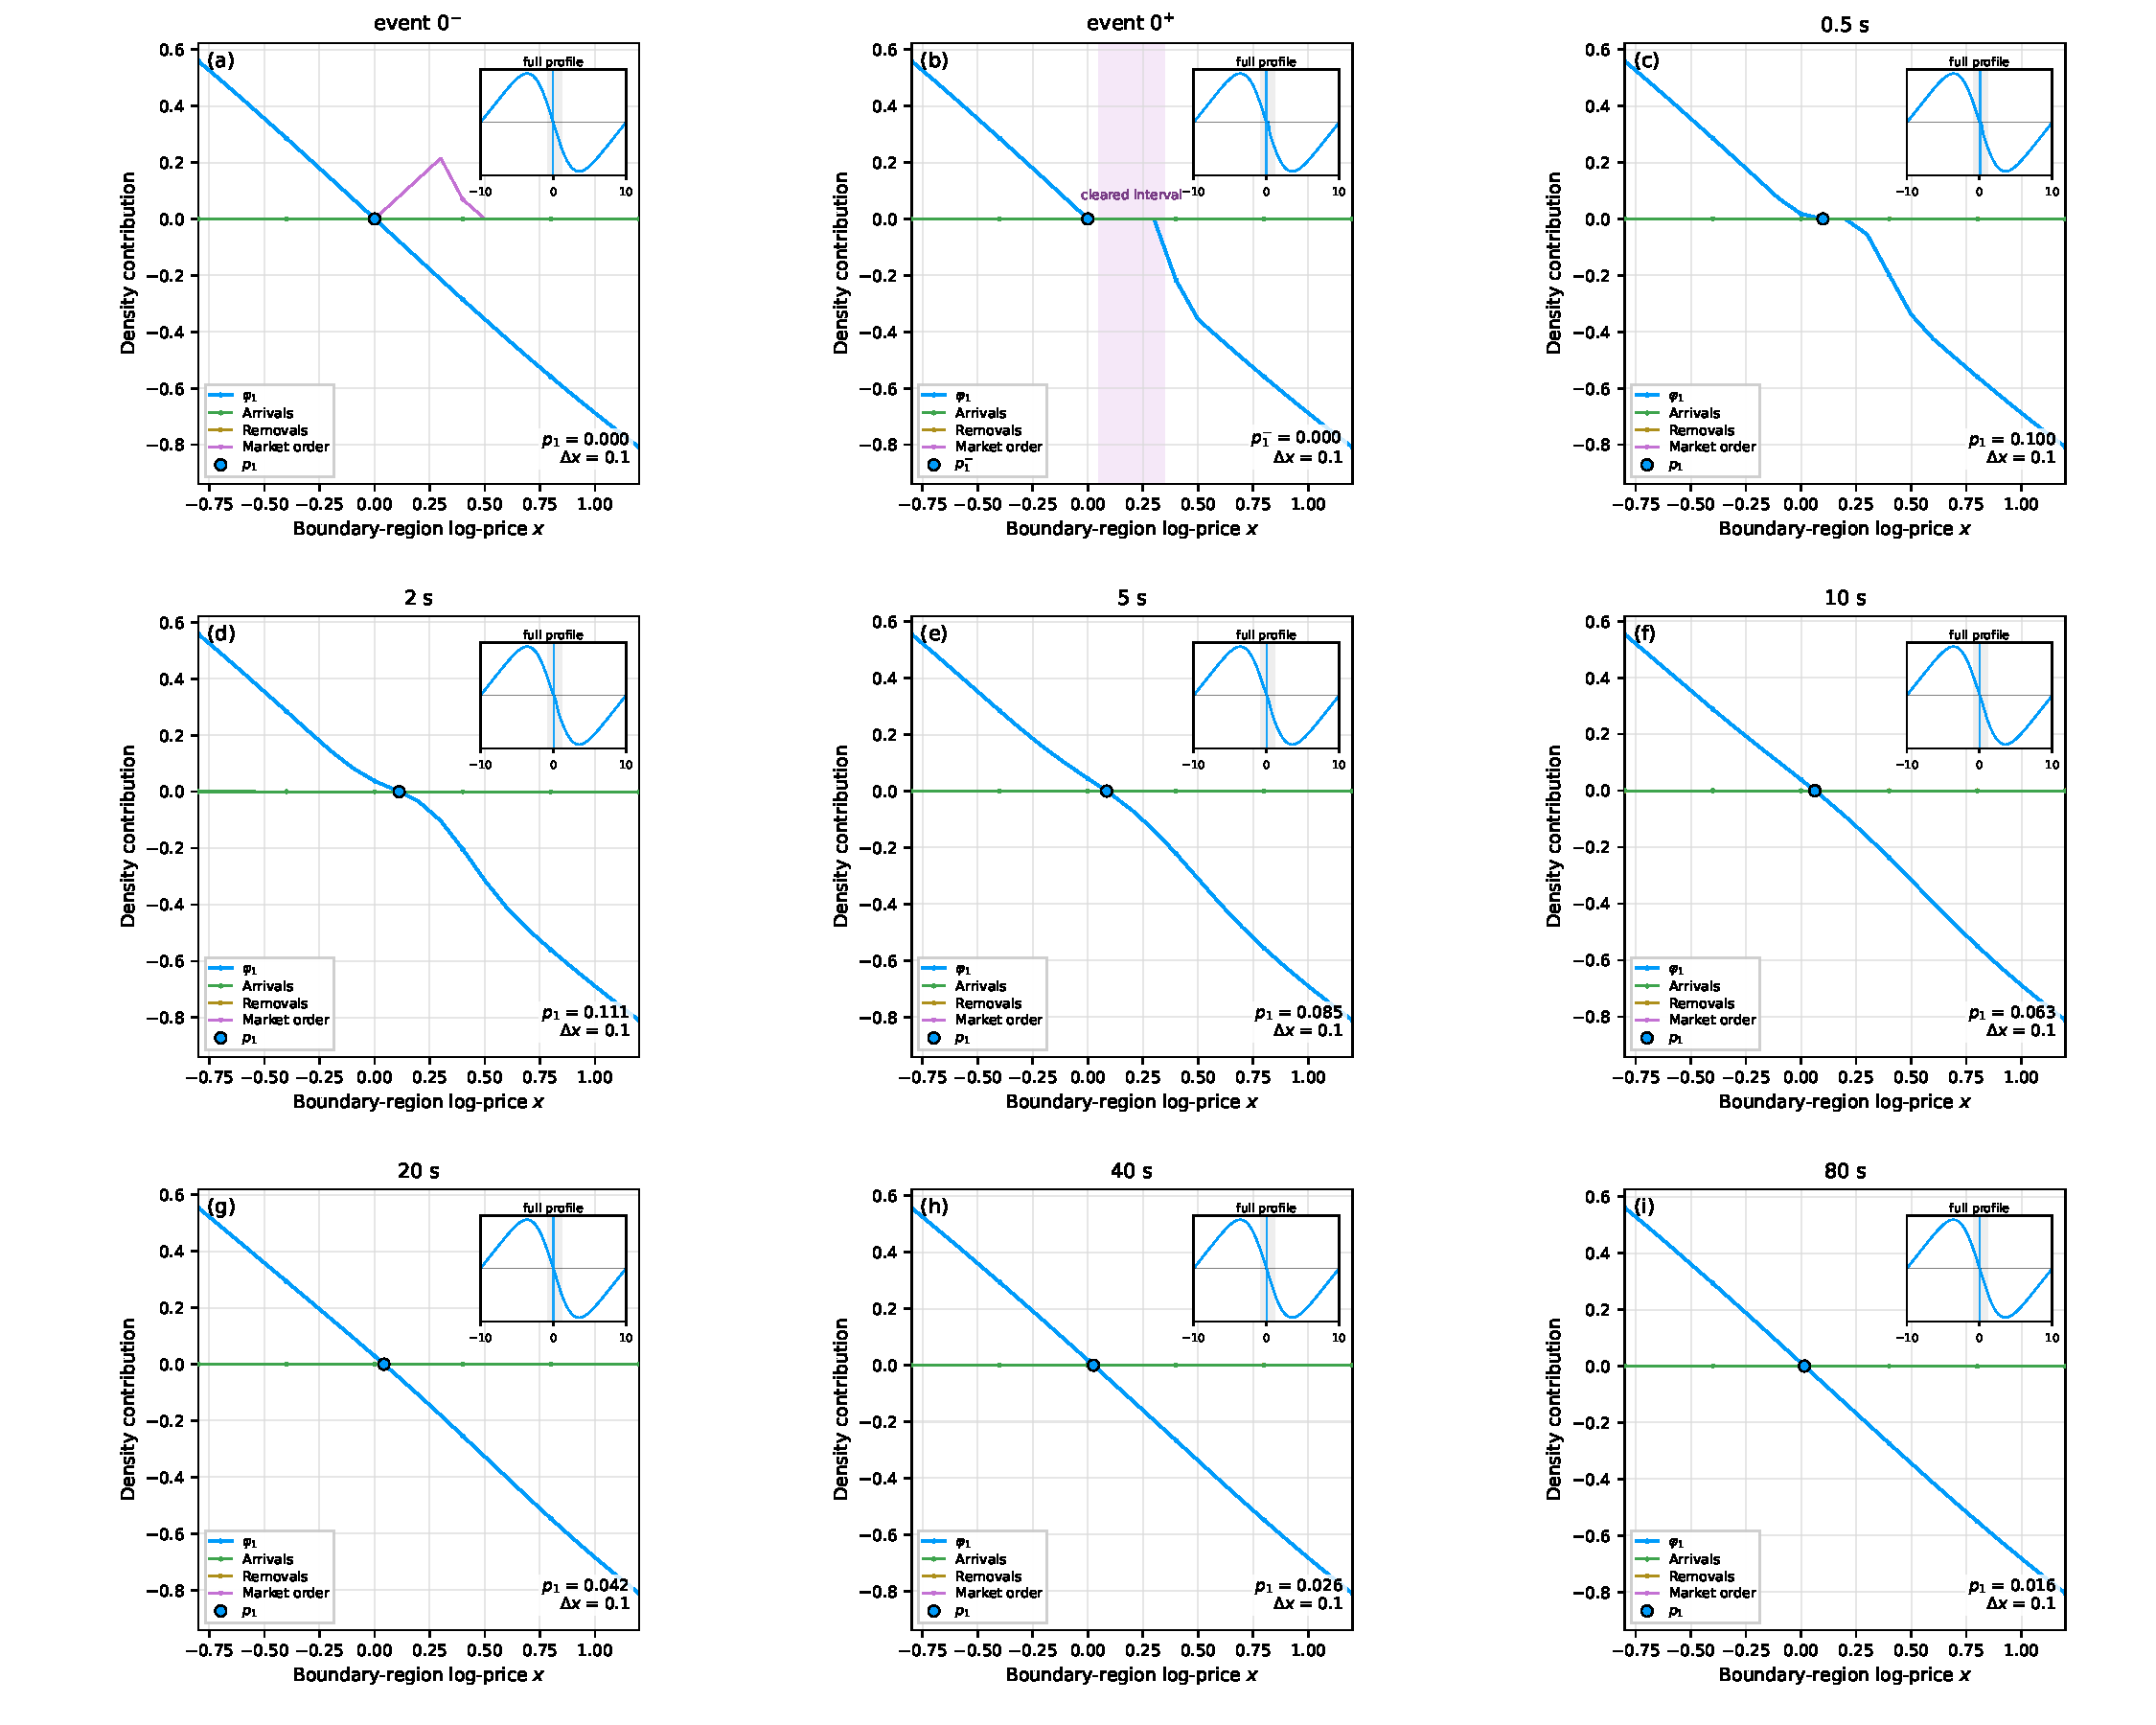
\includegraphics[width=\textwidth]{figures/figure-12-order-book-shock-recovery-v2.pdf}
\caption{\textbf{Fixed-time order-book shock recovery.} Nine snapshots follow
a buy market order in book 1 from the pre-event state $0^-$, through the
post-consumption state $0^+$, to $80$ seconds of fixed operational-time
evolution.  Blue is the signed density $\varphi_1$, green is the per-step
arrival contribution, gold is the per-step removal contribution, magenta is
the market-order density increment shown in panel (a), and the blue marker is the registered
reaction boundary.  The order consumes opposing liquidity from the boundary
outwards.  In panel (b) this creates a zero-density interval, so the marker is
the last registered boundary $p_1^-$; a unique simple zero is again registered
after the first completed step.  The accepted model has $\nu_1=\nu_2=0$, and
the gold curve is consequently zero in every panel.  Translation-mode coupling
to book 2 remains active and is retained in the numerical ledger but is not
drawn as an additional curve.  The registered boundary moves by $0.0997$ after
the first completed step, reaches $0.111$ at $2$ seconds and relaxes to a
residual displacement of $0.0160$ at $80$ seconds.  The price grid and
operational step are fixed.  All contribution curves use the same density
scale and are not independently rescaled.
The figure recovers the earlier panel structure without claiming a pointwise
replication of the Bauer et al. trajectory.}
\label{fig:fixed-time-shock-recovery}
\end{figure}
